\subsection{Comparing Source-Line Hints}
\label{sec:eval:recovery_ablation}

We compare six prompt settings on the same 60 new-test receipts.
The test uses 360 new Gemma responses from the same batch as the component
tests. All responses parse. Each setting keeps the full source and shares
the model, output limit, and filter.
The random index has about the same character length as the full index.

\begin{table}[t]

\centering

\caption{Source-line tests on 60 receipts. Each row uses the same model, source, output limit, and filter. Random hints have about the same character length as the index.}
\label{tab:recovery_index}

\small

\begin{tabular}{lrr}

\toprule

Context & Exact F1 & Normalized F1 \\

\midrule

Simple & 0.7917 & 0.8125 \\

Full index & 0.8351 & 0.8643 \\

Anchors only & 0.8351 & 0.8643 \\

Random index & 0.8167 & 0.8458 \\

Simple, no definitions & 0.8083 & 0.8292 \\

Full index, no definitions & 0.7470 & 0.7762 \\

\bottomrule

\end{tabular}

\end{table}

The full index leads Simple by 4.35 F1 points (95\% CI: 1.25 to 7.86).
Its Holm-corrected value is $p_H=0.065$ across five planned comparisons.
The full index and anchor lines alone have the same mean F1.
The full--random difference is 1.85 points
(CI: $[-0.65,4.52]$; $p_H=0.696$).
Removing field meanings from the full index lowers F1 by 8.81 points
(CI: $[4.23,13.39]$; $p_H=0.006$).
The Simple setting scores higher with field meanings removed in this batch.
These results show that field meanings help the indexed prompt choose values.

\begin{figure}[t]

\centering

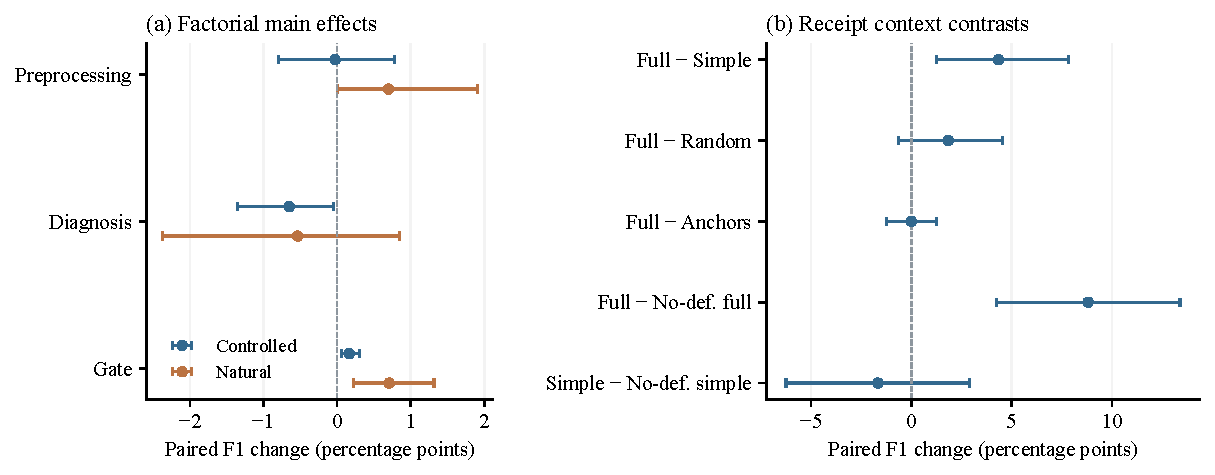
\includegraphics[width=0.98\textwidth]{figure/experiments/recovery_ablation.pdf}

\caption{Component and source-line tests. Points show mean paired F1 changes. Bars show 95\% CIs for each change. The component and receipt tests use separate Holm groups.}
\label{fig:recovery_ablation}

\end{figure}
